\documentclass[11pt,a4paper]{article}
\usepackage[margin=2.2cm]{geometry}
\usepackage{booktabs}
\usepackage{graphicx}
\usepackage{float}
\usepackage[table]{xcolor}
\usepackage{caption}
\usepackage{parskip}
\usepackage{fancyhdr}
\usepackage{longtable}
\usepackage{array}
\graphicspath{{../figures/}}
\captionsetup{font=small,labelfont=bf,width=0.92\textwidth}
\setlength{\parskip}{0.55em}
\setlength{\parindent}{0pt}
\pagestyle{fancy}
\fancyhf{}
\fancyhead[L]{\small\textit{Fault-detection analytics pack}}
\fancyhead[R]{\small\textit{regenerated data, 2026-11-12}}
\fancyfoot[C]{\small\thepage}
\renewcommand{\headrulewidth}{0.3pt}
\begin{document}

% ============================================================
% TITLE
% ============================================================

\begin{titlepage}
\centering
\vspace*{3.2cm}
{\LARGE\bfseries Fault-Detection Analytics Pack\par}
\vspace{0.5cm}
{\large Companion figures and verified numbers for the
dissertation writer\par}
\vspace{1.2cm}
{\large Regenerated-data era --- 2026-11-12\par}
\vspace{2.2cm}
\begin{center}
\texttt{\small
data/classdetectfault\_sim.csv\quad md5 cf24c7fbe993...\quad
5{,}365 rows\\[2pt]
data/detectfault\_sim.csv\quad md5 807df9dd62a4...\quad
9{,}503 rows\\[2pt]
branch \texttt{exp}\quad build 2026-11-12\_20-21-33}
\end{center}
\vfill
{\small Every figure and number in this pack is generated by
\texttt{src/analytics.py} from re-runnable reports; the
traceability appendix maps each one to its source.\par}
\end{titlepage}

% ============================================================
\section{Dataset and provenance}

The pack is built on the Python re-simulation of the corrected
161 kV / 120 km line (Z\textsubscript{1} = 0.080 + j0.390,
Z\textsubscript{0} = 0.228 + j1.352 $\Omega$/km, C\textsubscript{1}
= 12.74 nF/km). The classification dataset holds 5{,}365 rows
(3{,}000 fault rows in 375 eight-row location sweeps + 2{,}365
no-fault rows); the detection dataset holds 9{,}503 rows and is
31.6\% fault rows (45.8\% in the superseded original). The
scenario-level split assigns 134 of 671 scenarios (1{,}069 rows) to
the shared test partition of all eight models.

\begin{figure}[H]
\centering
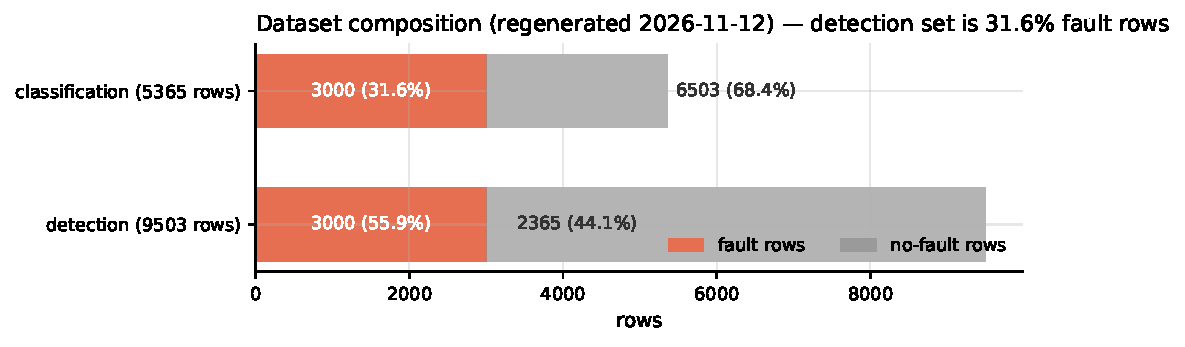
\includegraphics[width=0.88\textwidth]{fig03_dataset_composition.pdf}
\caption{Dataset composition. Where it goes: Section 4.2 (dataset presentation). Source: data files; counts asserted at build time.}
\end{figure}


\begin{figure}[H]
\centering
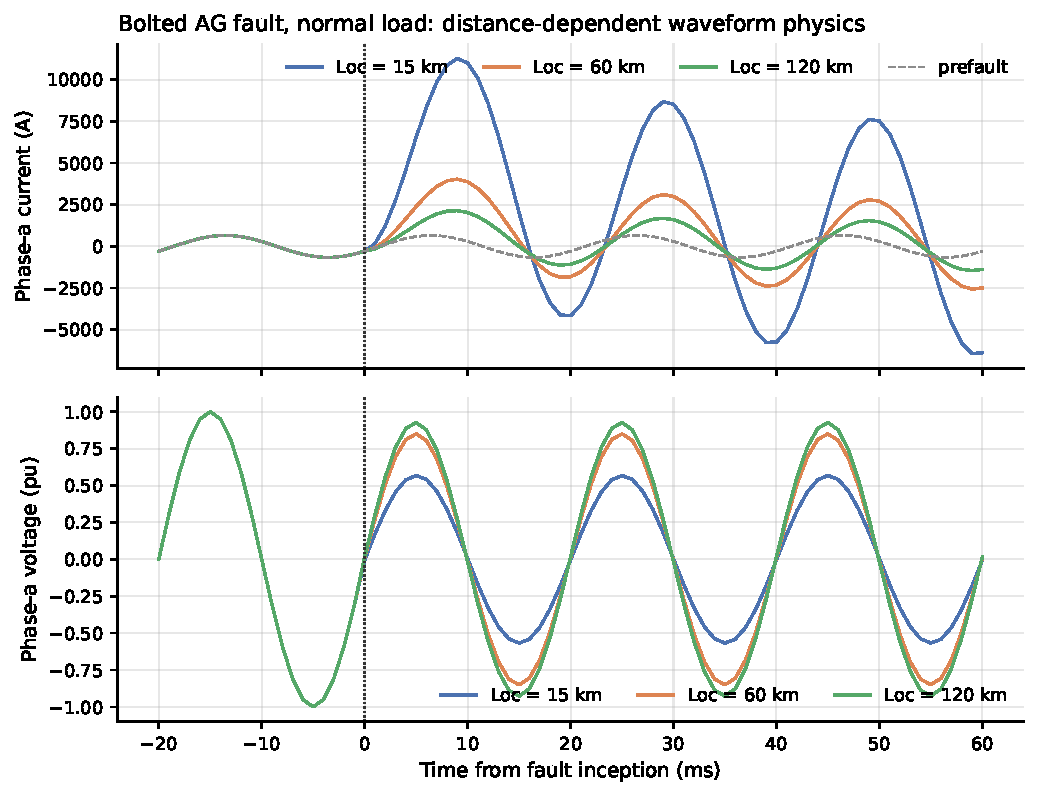
\includegraphics[width=0.88\textwidth]{fig01_waveforms_distance.pdf}
\caption{Distance-dependent waveform physics, now present in the regenerated data (the original data was flat in location). Fault current decays 4.76 to 0.89 kA and the faulted-phase voltage sag relaxes 0.568 to 0.928 pu across 15 to 120 km. Where it goes: Section 3.5.5 (dataset generation) and the R10 waveform discussion. Source: src/simulate.py, bolted AG, normal load.}
\end{figure}


\begin{figure}[H]
\centering
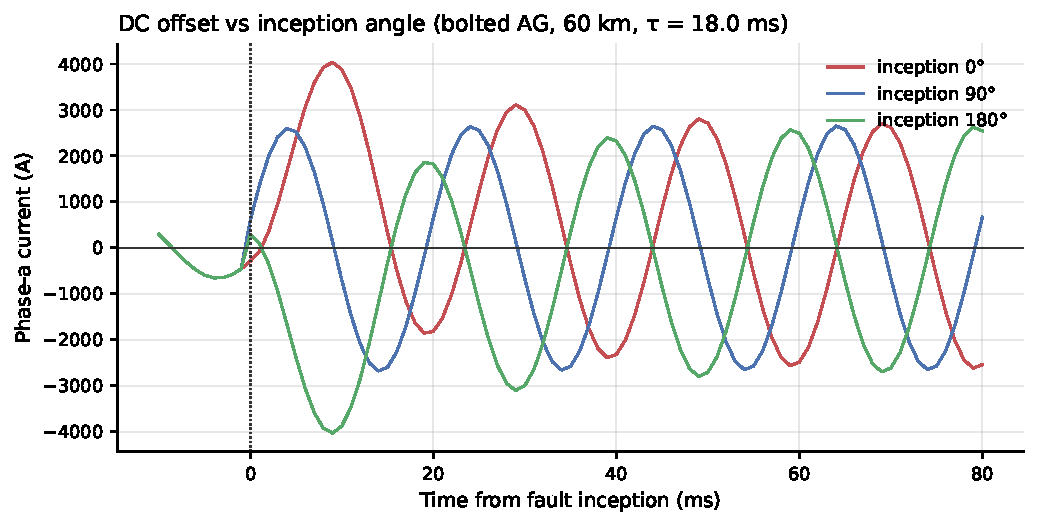
\includegraphics[width=0.88\textwidth]{fig02_dc_offset.pdf}
\caption{DC offset vs inception angle: the offset peaks at the voltage-zero crossings and vanishes near the voltage peak, decaying with the positive-sequence loop time constant. Where it goes: Section 3.5.5 and R10. Source: src/simulate.py.}
\end{figure}


\section{Conventional relay baseline}

The relay is a numerical distance relay deciding on six loop
impedances (three residual-compensated ground loops
$|V_p|/|I_p + k_0\,3I_0|$, $k_0 = 0.8140 + j0.0405$, and three
phase-phase loops) evaluated as steady-state phasor quantities. The
Zone 1 reach is $0.80 \times |Z_1| \times 120$ km =
38.22~$\Omega$. Its profile on the regenerated data:
true-negative rate 100\%, trip rate 49.2\% of fault rows, overall
accuracy 0.7158 (all rows) / 0.7568 (common test rows) --- secure but
incomplete.

\begin{figure}[H]
\centering
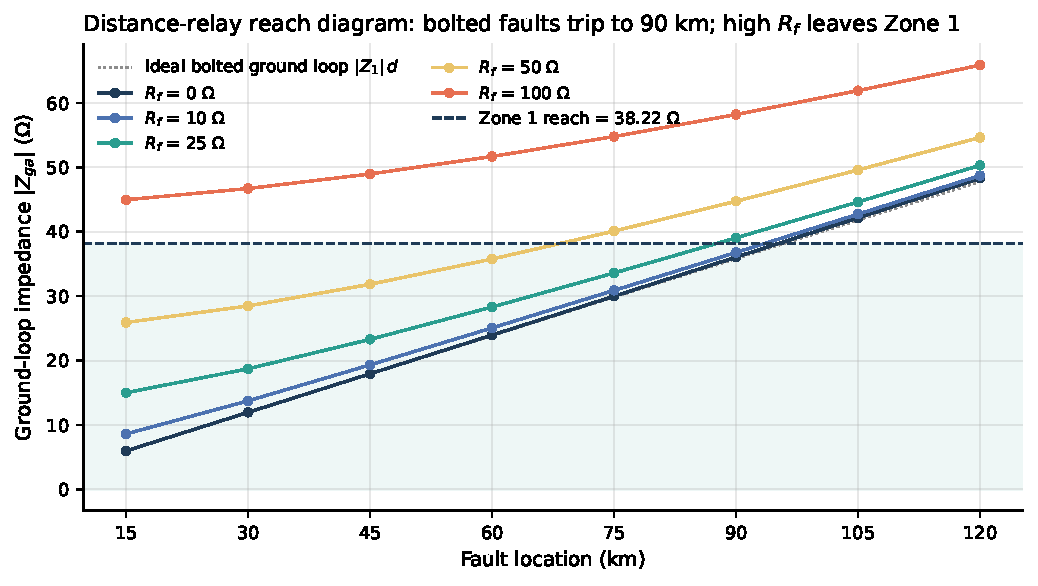
\includegraphics[width=0.88\textwidth]{fig04_reach_diagram.pdf}
\caption{Reach diagram. Bolted faults trip to 90 km ($|Z_1|d = 36.0$ $\Omega$ < 38.22 $\Omega$); 105 and 120 km fall beyond Zone 1, and high-resistance faults leave Zone 1 at every location. Where it goes: Section 3.9.4 (relay detection logic). Source: src/simulate.py loop impedances + src/relay.py reach.}
\end{figure}


\begin{figure}[H]
\centering
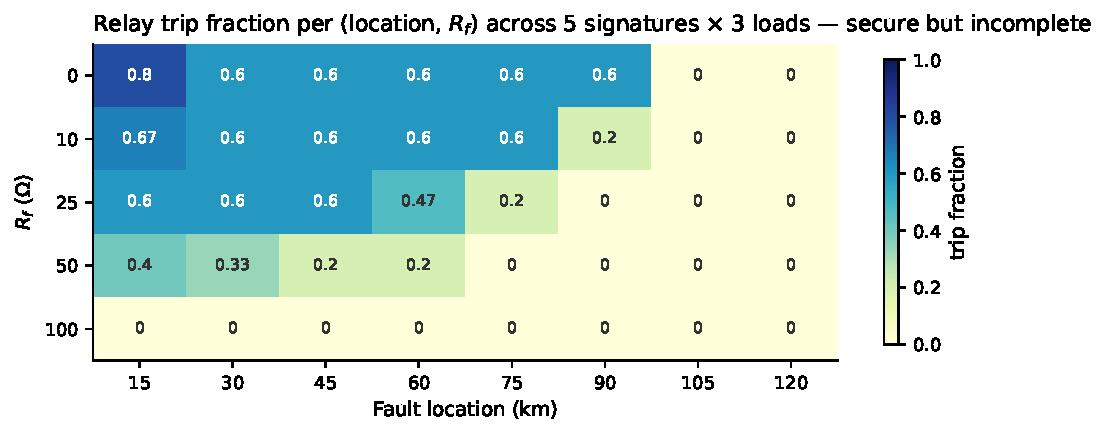
\includegraphics[width=0.88\textwidth]{fig05_relay_trip_heatmap.pdf}
\caption{Trip fraction across the full factorial (5 signatures x 3 load levels; the inception angle does not enter the steady-state decision). The white corners --- high $R_f$, far faults --- are exactly the regime the learned models cover. Where it goes: Section 4.x, H1 discussion. Source: src/simulate.py.}
\end{figure}


\section{Classification performance (Table 4.3, H1, H2)}

All values carry bootstrap SDs (2{,}000 resamples, seed 42) on the
1{,}069 common test rows. The weakest cell in the table is the RNN on
phase A (accuracy 0.9280); the LSTM attains 1.0 on every target.

\begin{table}[H]
\centering
\footnotesize
\setlength{\tabcolsep}{3.5pt}
\begin{tabular}{@{}lrlrrrr@{}}
\toprule
model & $n$ & accuracy & recall & F1 & robustness & latency (ms) \\
\midrule
ann & 1069 & 0.9944 ± 0.0024 & 0.9900 ± 0.0041 & 0.9950 ± 0.0020 & 0.9836 $\pm$ 0.0009 & 0.0011 $\pm$ 0.0002 \\
cnn & 1069 & 0.9981 ± 0.0014 & 0.9967 ± 0.0023 & 0.9983 ± 0.0012 & 0.9853 $\pm$ 0.0006 & 0.0557 $\pm$ 0.0070 \\
dtr & 1069 & 0.9972 ± 0.0016 & 0.9950 ± 0.0029 & 0.9975 ± 0.0015 & 0.9383 $\pm$ 0.0046 & 0.0007 $\pm$ 0.0001 \\
knn & 1069 & 0.9963 ± 0.0019 & 0.9933 ± 0.0034 & 0.9967 ± 0.0017 & 0.9819 $\pm$ 0.0009 & 0.0148 $\pm$ 0.0027 \\
lstm & 1069 & 1.0000 ± 0.0000 & 1.0000 ± 0.0000 & 1.0000 ± 0.0000 & 1.0000 $\pm$ 0.0000 & 204.91 $\pm$ 103.85 \\
pinn & 1069 & 0.9972 ± 0.0016 & 0.9950 ± 0.0028 & 0.9975 ± 0.0014 & 0.9840 $\pm$ 0.0011 & 0.0038 $\pm$ 0.0005 \\
rnn & 1069 & 0.9935 ± 0.0024 & 0.9883 ± 0.0044 & 0.9941 ± 0.0023 & 0.9842 $\pm$ 0.0011 & 0.0008 $\pm$ 0.0000 \\
svm & 1069 & 0.9991 ± 0.0009 & 0.9983 ± 0.0016 & 0.9992 ± 0.0009 & 0.9804 $\pm$ 0.0010 & 0.0011 $\pm$ 0.0002 \\
relay & 1069 & 0.7568 ± 0.0130 & 0.5667 ± 0.0201 & 0.7234 ± 0.0165 & n/a & 10.00 $\pm$ 0.00 \\
relay (all rows) & 5365 & 0.7158 ± 0.0063 & 0.4917 ± 0.0091 & 0.6592 ± 0.0082 & n/a & 10.00 $\pm$ 0.00 \\
\bottomrule
\end{tabular}
\caption{Table 4.3 (regenerated), overall rows. Relay ``all rows''
covers the full 5{,}365-row dataset. Source: outputs/table\_4\_3
(report 2026-11-12\_19-43-50).}
\end{table}

\begin{figure}[H]
\centering
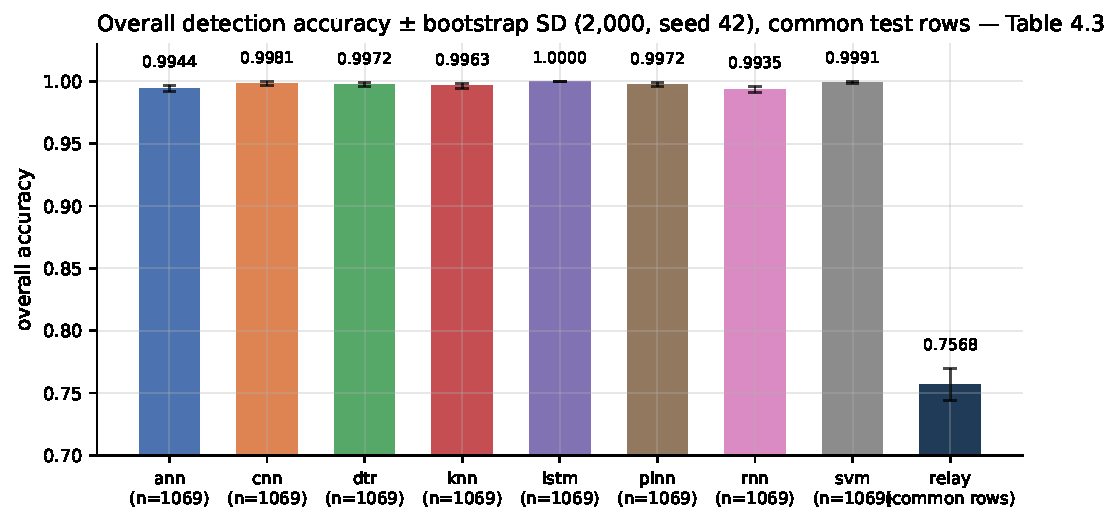
\includegraphics[width=0.88\textwidth]{fig06_accuracy_bars.pdf}
\caption{Overall detection accuracy with bootstrap SDs. Where it goes: Section 4.x, Table 4.3 discussion. Source: table\_4\_3.csv.}
\end{figure}


\begin{figure}[H]
\centering
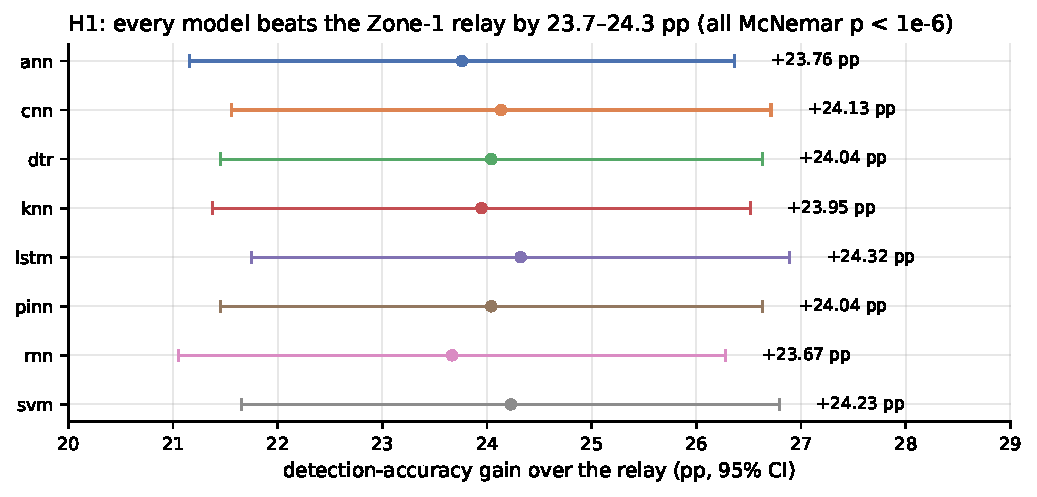
\includegraphics[width=0.88\textwidth]{fig08_h1_forest.pdf}
\caption{H1 forest plot: accuracy gain over the relay with 95\% CIs; Cochran's Q = 1906.85 (df = 8, $p < 10^{-6}$). Where it goes: Section 4.x, H1. Source: hypothesis results CSV.}
\end{figure}


\begin{figure}[H]
\centering
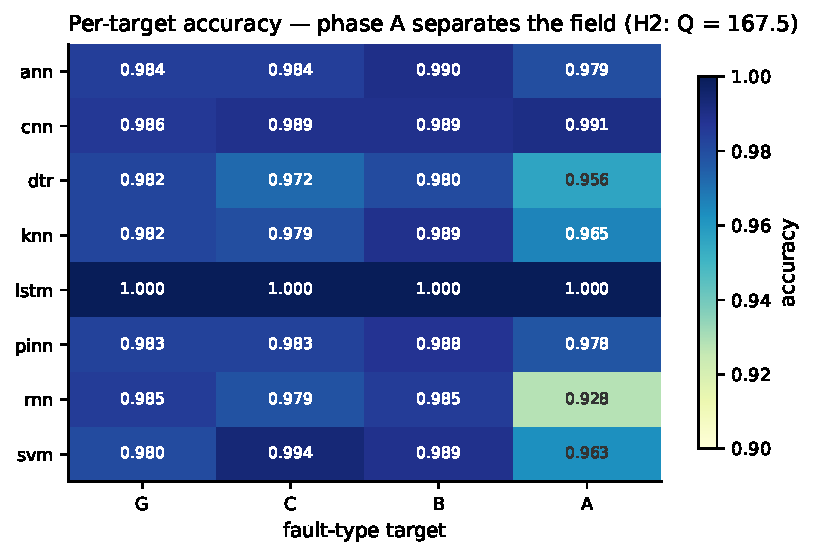
\includegraphics[width=0.88\textwidth]{fig07_per_target_heatmap.pdf}
\caption{Per-target accuracy. Per-target Cochran's Q: G: Q = 40.04, C: Q = 60.13, B: Q = 37.68, A: Q = 167.49; under Holm correction the LSTM is significantly best on G/C/B and, with CNN, on phase A. Where it goes: Section 4.x, H2. Source: hypothesis results CSV.}
\end{figure}


\section{Latency and noise robustness (H3, H4)}

\begin{figure}[H]
\centering
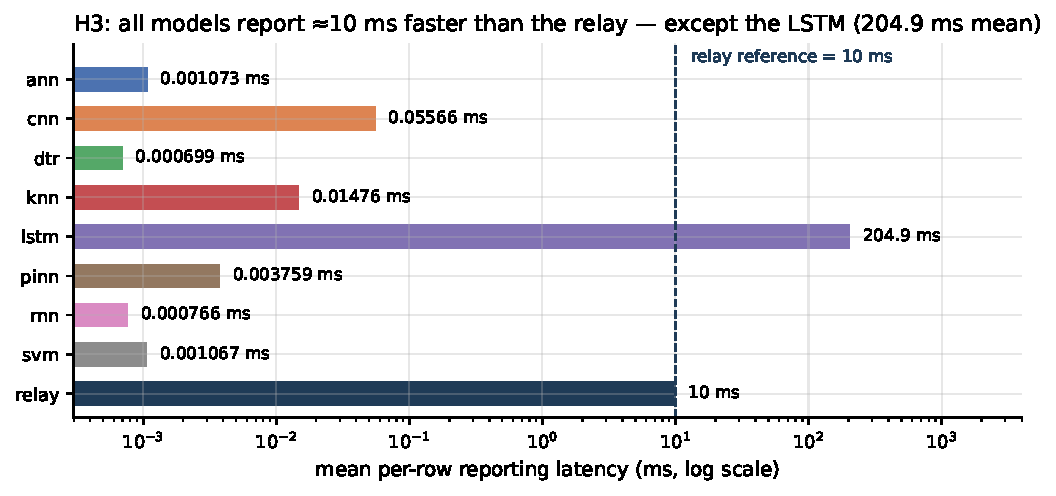
\includegraphics[width=0.88\textwidth]{fig09_latency.pdf}
\caption{Reporting latency (log scale). Every model reports faster than the relay's 10 ms reference by essentially the full margin (Hodges--Lehmann $\approx -10$ ms); the LSTM reports 188.75 ms slower (95\% CI [178.5, 197.0], mean 204.9 ms). Where it goes: Section 4.x, H3 --- replaces the stale ``270 ms'' sentence. Source: table\_4\_3.csv + hypothesis results CSV.}
\end{figure}


\begin{figure}[H]
\centering
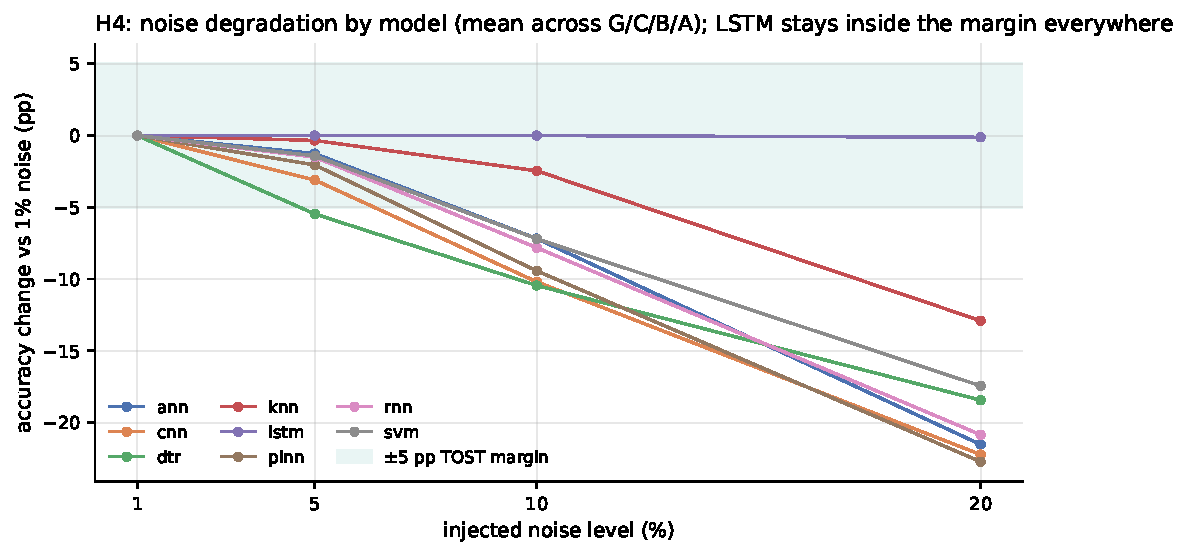
\includegraphics[width=0.88\textwidth]{fig10_robustness_curves.pdf}
\caption{Accuracy change vs the 1\% noise baseline, mean across targets. The shaded band is the pre-declared 5 pp TOST equivalence margin: the LSTM is equivalent at every level, KNN up to 10\% on all targets, the others break at 20\%; CNN and PINN are not equivalent on phase A even at 5\%. Where it goes: Section 4.x, H4. Source: robustness\_*.csv (2026-11-12 rows).}
\end{figure}


\section{Fault location and scenario structure (H5, R9)}

Location accuracy is measured on the 600 fault scenarios of the
common test set (MAE as \% of the 120 km line).

\begin{table}[H]
\centering
\small
\begin{tabular}{@{}lrrr@{}}
\toprule
model & locations & MAE (km) & MAE (\% of 120 km) \\
\midrule
lstm & 8 & 0.46 & 0.380 \\
dtr & 8 & 2.23 & 1.858 \\
knn & 8 & 5.18 & 4.319 \\
cnn & 8 & 9.68 & 8.066 \\
ann & 8 & 13.54 & 11.282 \\
svm & 8 & 13.61 & 11.345 \\
rnn & 8 & 15.23 & 12.692 \\
pinn & 8 & 15.88 & 13.237 \\
\bottomrule
\end{tabular}
\caption{H5 fault-location MAE, recomputed from the Loc columns of
the prediction files and asserted against the hypothesis report
(within 0.05 pp). Source: predictions\_*.csv.}
\end{table}

\begin{figure}[H]
\centering
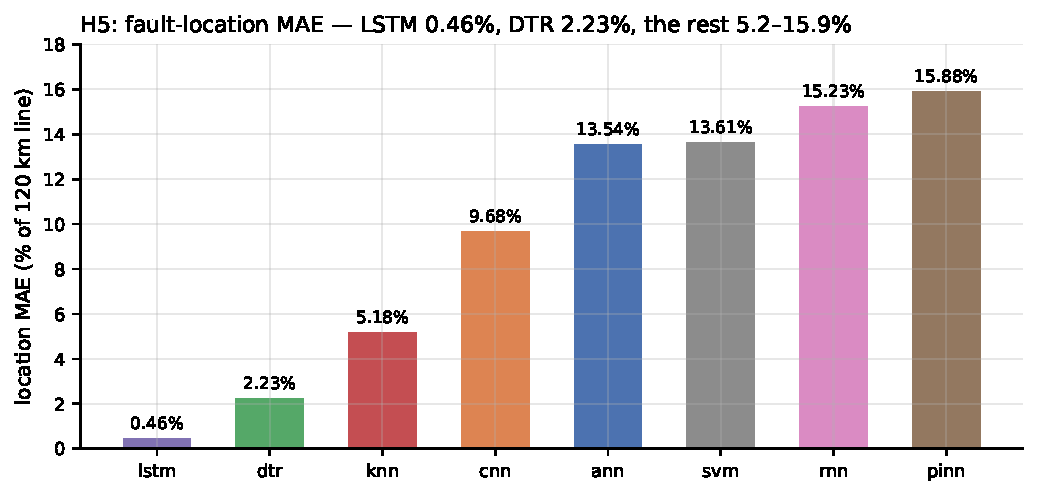
\includegraphics[width=0.88\textwidth]{fig11_mae_bars.pdf}
\caption{Location MAE ranking. Where it goes: Section 4.x, H5. Source: prediction files (asserted).}
\end{figure}


\begin{figure}[H]
\centering
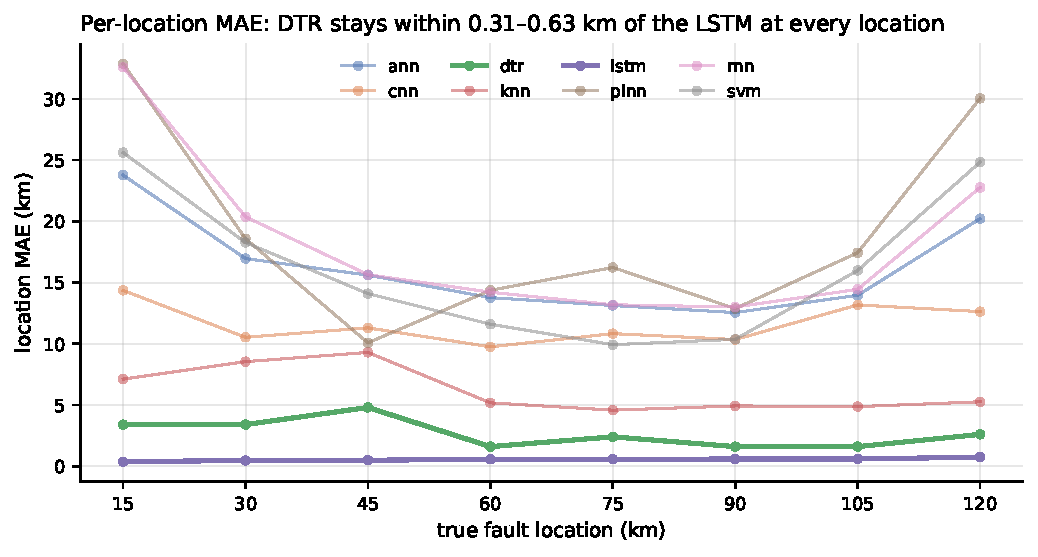
\includegraphics[width=0.88\textwidth]{fig12_mae_by_location.pdf}
\caption{Per-location MAE. The DTR stays within 0.31--0.63 km of the LSTM at every location (all Holm-adjusted $p < 10^{-6}$); every other model trails by 3.3--30.9 km. Friedman all-locations $\chi^2$ = 2338.9, Kendall's W = 0.557. Where it goes: Section 4.x, H5. Source: prediction files.}
\end{figure}


\begin{figure}[H]
\centering
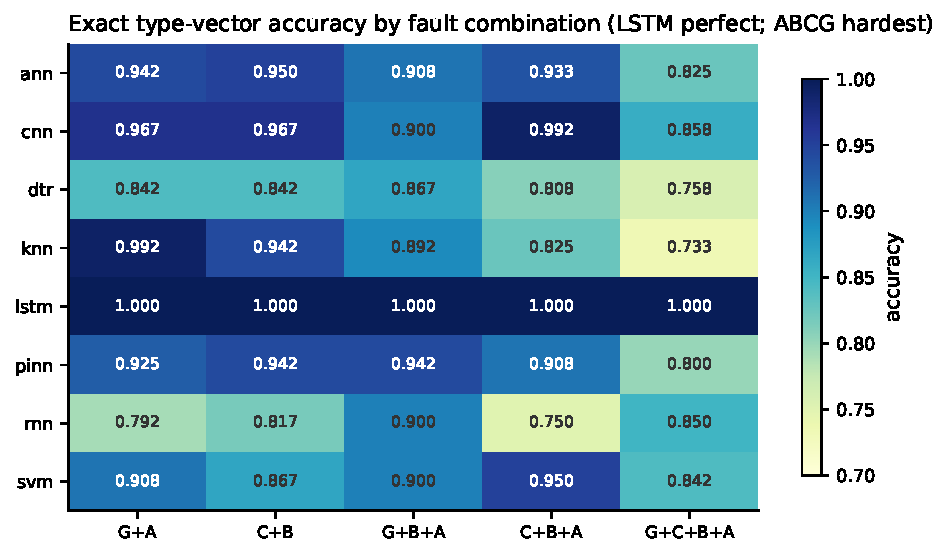
\includegraphics[width=0.88\textwidth]{fig13_combination_heatmap.pdf}
\caption{Exact type-vector accuracy by fault combination; the relay row is structurally inapplicable (binary trip output) and is omitted. Where it goes: Section 4.x, combination-accuracy discussion. Source: combination results CSV.}
\end{figure}


\begin{figure}[H]
\centering
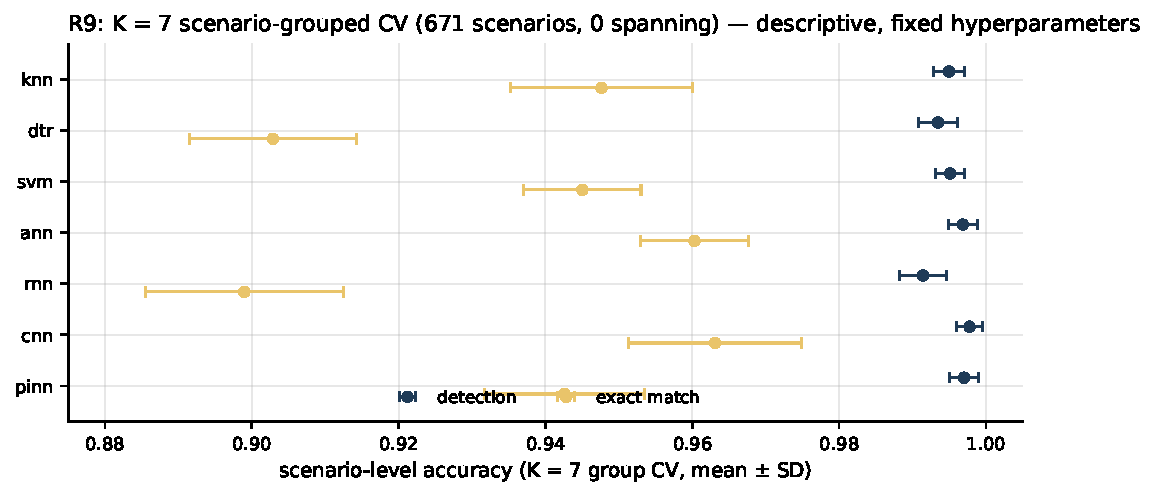
\includegraphics[width=0.88\textwidth]{fig14_cv.pdf}
\caption{Scenario-grouped K = 7 CV (descriptive, fixed hyperparameters): detection 0.9914--0.9978, exact match 0.8990--0.9631. Where it goes: Section 3.12.1 / 4.x (R9). Source: cv\_results CSV.}
\end{figure}


\begin{table}[H]
\centering
\small
\begin{tabular}{@{}lrr@{}}
\toprule
model & detection acc. & exact-match acc. \\
\midrule
knn & 0.9950 $\pm$ 0.0021 & 0.9476 $\pm$ 0.0124 \\
dtr & 0.9935 $\pm$ 0.0027 & 0.9029 $\pm$ 0.0114 \\
svm & 0.9952 $\pm$ 0.0020 & 0.9450 $\pm$ 0.0080 \\
ann & 0.9968 $\pm$ 0.0020 & 0.9603 $\pm$ 0.0073 \\
rnn & 0.9914 $\pm$ 0.0032 & 0.8990 $\pm$ 0.0135 \\
cnn & 0.9978 $\pm$ 0.0018 & 0.9631 $\pm$ 0.0117 \\
pinn & 0.9970 $\pm$ 0.0020 & 0.9426 $\pm$ 0.0109 \\
\bottomrule
\end{tabular}
\caption{CV means $\pm$ SD across the 7 scenario-grouped folds.
Source: outputs/scenario\_cv (report 2026-11-12\_17-25-03).}
\end{table}

A scenario-level leakage audit found zero spanning scenarios for all
nine methods (models touch 134 of 671 test scenarios; the relay, which
trains on nothing, covers all 671).

\section{Writer's companion}

\subsection{Key takeaways, keyed to the chapter}
\begin{itemize}
\item \textbf{\S3.3.1} --- correct the line-charging figure to
4.15 MVAr (120 km section) / 10.28 MVAr (297.4 km route); keep the
10.8 kA bolted three-phase cross-check.
\item \textbf{\S3.3} --- insert the declared auxiliary assumptions
(X/R = 10; 0.95 pf constant-impedance load at 40/75/100\% of 750 A;
$C_0 = 0.75\,C_1$; $Z_0$ source = $Z_1$ source; bolted ground;
$R_f = 0 \equiv 1$ m$\Omega$; EMF calibration) and the load-bus
operating points 0.931/0.862/0.815 pu.
\item \textbf{\S3.5.5} --- new design space: 375 sweeps x 8
locations = 3{,}000 fault rows; datasets 5{,}365 / 9{,}503 rows;
detection set 31.6\% fault rows; event-sweep model caveat.
\item \textbf{\S3.8.2/3.12.1} --- 671 scenarios, shared
scenario-level split (134 test scenarios / 1{,}069 rows), K = 7 CV is
descriptive only.
\item \textbf{\S3.9.4} --- relay measurement chain: six loops,
complex $k_0$, Zone 1 = 38.22 $\Omega$, steady-state phasor
semantics; secure-but-incomplete profile (TN 100\%, TP 49.2\%).
\item \textbf{\S4.x} --- Table 4.3, H1--H5 numbers from this pack;
LSTM latency gap is $\approx$189 ms, not 270 ms.
\end{itemize}

\subsection{Do NOT transcribe (superseded numbers)}
\begin{itemize}
\item ``12{,}000 scenarios / 14{,}400 rows / 2{,}400 held-out
scenarios / 7{,}861 rows''; ``45.8\% fault rows''; ``5{,}496 fault
rows / 685 sweeps + 4 truncated''.
\item ``24{,}000 fault rows'' (design-space double-count).
\item ``$\approx$30.9 MVAr line charging'' ($\sqrt{3}$ slip).
\item ``LSTM latency gap $\approx$ 270 ms''.
\item Any accuracy, p-value, latency or table cell computed from the
original datasets.
\item Old relay narrative (``0.9+ detection accuracy'').
\item Old absolute waveform claims (44 A no-fault currents, 4\% of
nominal faulted-phase voltage, 0.62 prefault peak).
\end{itemize}

\subsection{Traceability appendix}

\begin{longtable}{@{}p{3.2cm}p{11.4cm}@{}}
\toprule
\textbf{tag} & \textbf{source} \\
\midrule
\endhead
SIM & \texttt{src/simulate.py} imported directly; 8-point
verification battery all PASS (outputs/simulate/report\_2026-11-12\_16-09-04.txt); datasets md5-identical across runs \\
REL & outputs/relay/report\_2026-11-12\_16-20-30.txt \\
T43 & outputs/table\_4\_3/report\_2026-11-12\_19-43-50.txt \\
HYP & outputs/hypothesis\_tests/report\_2026-11-12\_17-08-01.txt \\
CV & outputs/scenario\_cv/report\_2026-11-12\_17-25-03.txt \\
COMB & outputs/combination\_accuracy/report\_2026-11-12\_17-25-01.txt \\
LEAK & outputs/leakage\_audit/report\_2026-11-12\_17-25-01.txt \\
ROB & outputs/\textless model\textgreater/robustness\_\textless
model\textgreater{}.csv (2026-11-12 rows) \\
\bottomrule
\end{longtable}

\end{document}
